\documentclass{beamer}

% Encoding and language support
\usepackage[T2A]{fontenc}
\usepackage[utf8]{inputenc}
\usepackage[russian]{babel}

% Packages for math and graphics
\usepackage{amsmath}
\usepackage{graphicx}
\usepackage{booktabs} % For better tables
\usepackage{ragged2e} % For text alignment

% Minimalist theme
\usetheme{default}

% Black-and-white color scheme
\setbeamercolor{background canvas}{bg=white}
\setbeamercolor{normal text}{fg=black}
\setbeamercolor{title}{fg=black}
\setbeamercolor{author}{fg=black}
\setbeamercolor{date}{fg=black}
\setbeamercolor{frametitle}{fg=black}
\setbeamercolor{itemize item}{fg=black}
\setbeamercolor{itemize subitem}{fg=black}
\setbeamercolor{enumerate item}{fg=black}

\setbeamertemplate{title page}{
	\vspace*{0.5cm}
	\begin{center}
		
\includegraphics[height=1.1cm]{logo.jpg} % Логотип (можно удалить)
		\vskip0.5cm
		
		{\usebeamerfont{title}\bfseries\large\inserttitle\par}
		\vskip0.8cm
		
		{\usebeamerfont{author}\small
			\textbf{Кромачев М.А.}, гр. 5030102/10201\par}
		\vskip0.3cm
		
		{\usebeamerfont{institute}\footnotesize
			СПбПУ Петра Великого\par
			Физико-механический институт\par}
		\vskip0.8cm
		
		{\usebeamerfont{date}\footnotesize
			Научный руководитель: доц., к.ф.-м.н. И.Е. Ануфриев\par
			\insertdate\par}
	\end{center}
}

% Custom frame title without numbers
\setbeamertemplate{frametitle}{
	\vspace*{0.3cm}
	\begin{beamercolorbox}[wd=\textwidth]{frametitle}
		\usebeamerfont{frametitle}\insertframetitle
	\end{beamercolorbox}
	\vspace*{0.2cm}
}

% Add page number in bottom right corner (except title page)
\setbeamertemplate{footline}{
	\ifnum\insertframenumber=1\else% Skip title page
	\hfill\scriptsize\insertframenumber/\inserttotalframenumber\hspace*{0.5cm}\vspace{0.5cm}
	\fi%
}

% Itemize style
\setbeamertemplate{itemize item}{\color{black}$\bullet$}
\setbeamertemplate{itemize subitem}{\color{black}$\circ$}

% Text alignment
\setbeamertemplate{blocks}[rounded][shadow=false]
\justifying

% Remove navigation symbols
\setbeamertemplate{navigation symbols}{}

\title{Децентрализованное решение задачи о назначениях целей группе роботов}
\author{}
\date{\today}

\begin{document}
	
	\begin{frame}[plain]
		\titlepage
	\end{frame}

	\begin{frame}
		\frametitle{Содержание}
		\begin{itemize}
			\item Сущность задачи
			\item Обзор возможных робототехнических систем
			\item Положения, выносимые на защиту
			\item Формальная постановка задачи
			\item Венгерский метод
			\item Алгоритм аукциона
			\item Модификация алгоритма аукциона
			\item Результаты экспериментов
			\item Выводы и перспективы
		\end{itemize}
	\end{frame}
	
	\begin{frame}
	    \frametitle{Сущность задачи}
	    \begin{columns}[T]
	        \begin{column}{0.5\textwidth}
	            \begin{itemize}
	                \item Цели \raisebox{-0.3em}{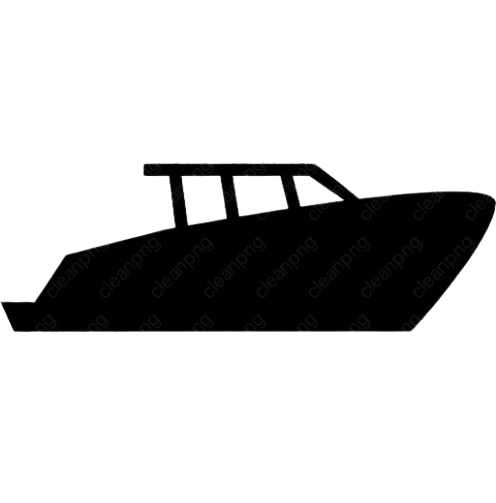
\includegraphics[width=0.5cm]{3.png}}  
	                \item Роботы {
\includegraphics[width=0.5cm]{2.jpg}}  
	                \begin{itemize}
	                    \item Радиус связи
	                    \item Область видимости
	                \end{itemize}
	                \item Центр управления \raisebox{-0.1em}{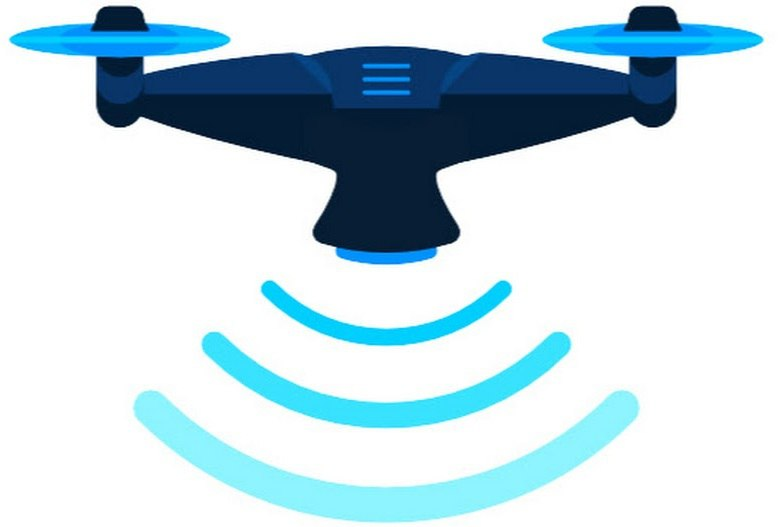
\includegraphics[width=0.5cm]{1.jpg}}  
	                \item Погрешность определения координат целей
	            \end{itemize}
	        \end{column}
	        \begin{column}{0.6\textwidth}
	            \centering
		 \hspace*{-1.5cm} % Отрицательный отступ для смещения влевоы
	            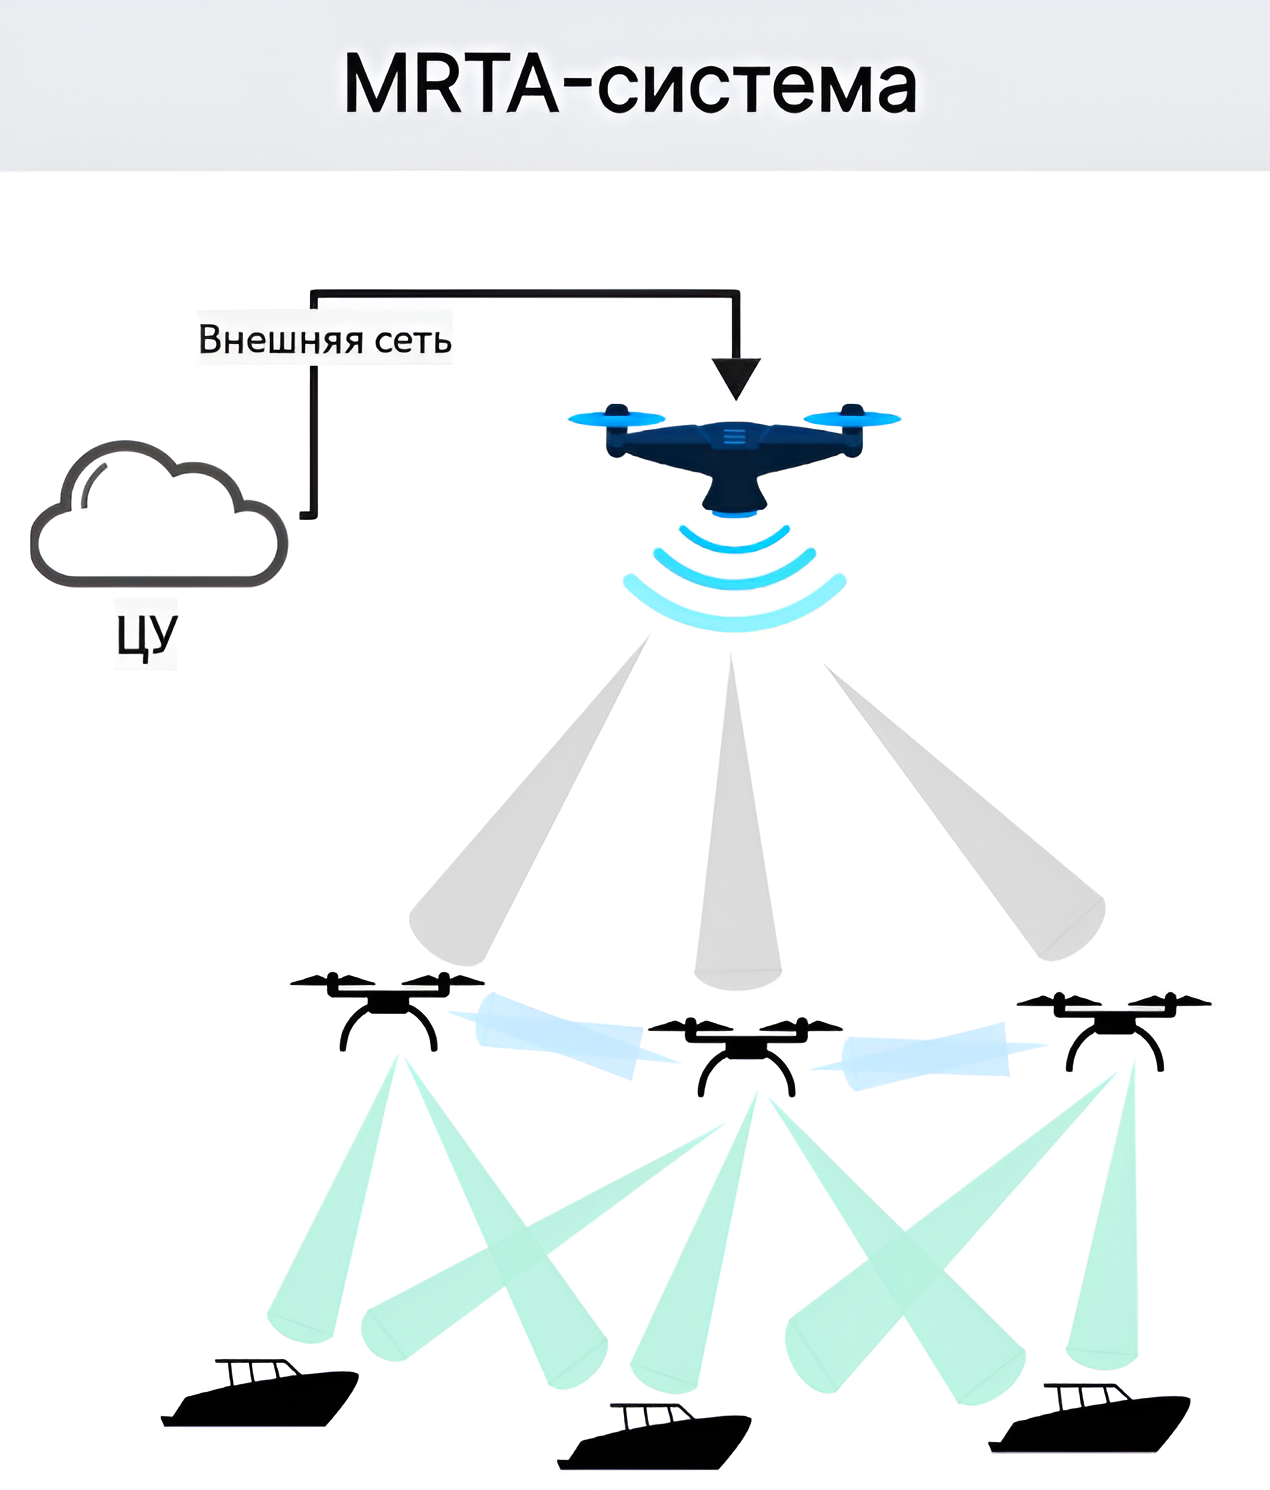
\includegraphics[width=\textwidth,height=0.85\textheight,keepaspectratio]{mrta1.png}
	        \end{column}
	    \end{columns}
	\end{frame}

	\begin{frame}
		\frametitle{Обзор возможных робототехнических систем}
		\centering
		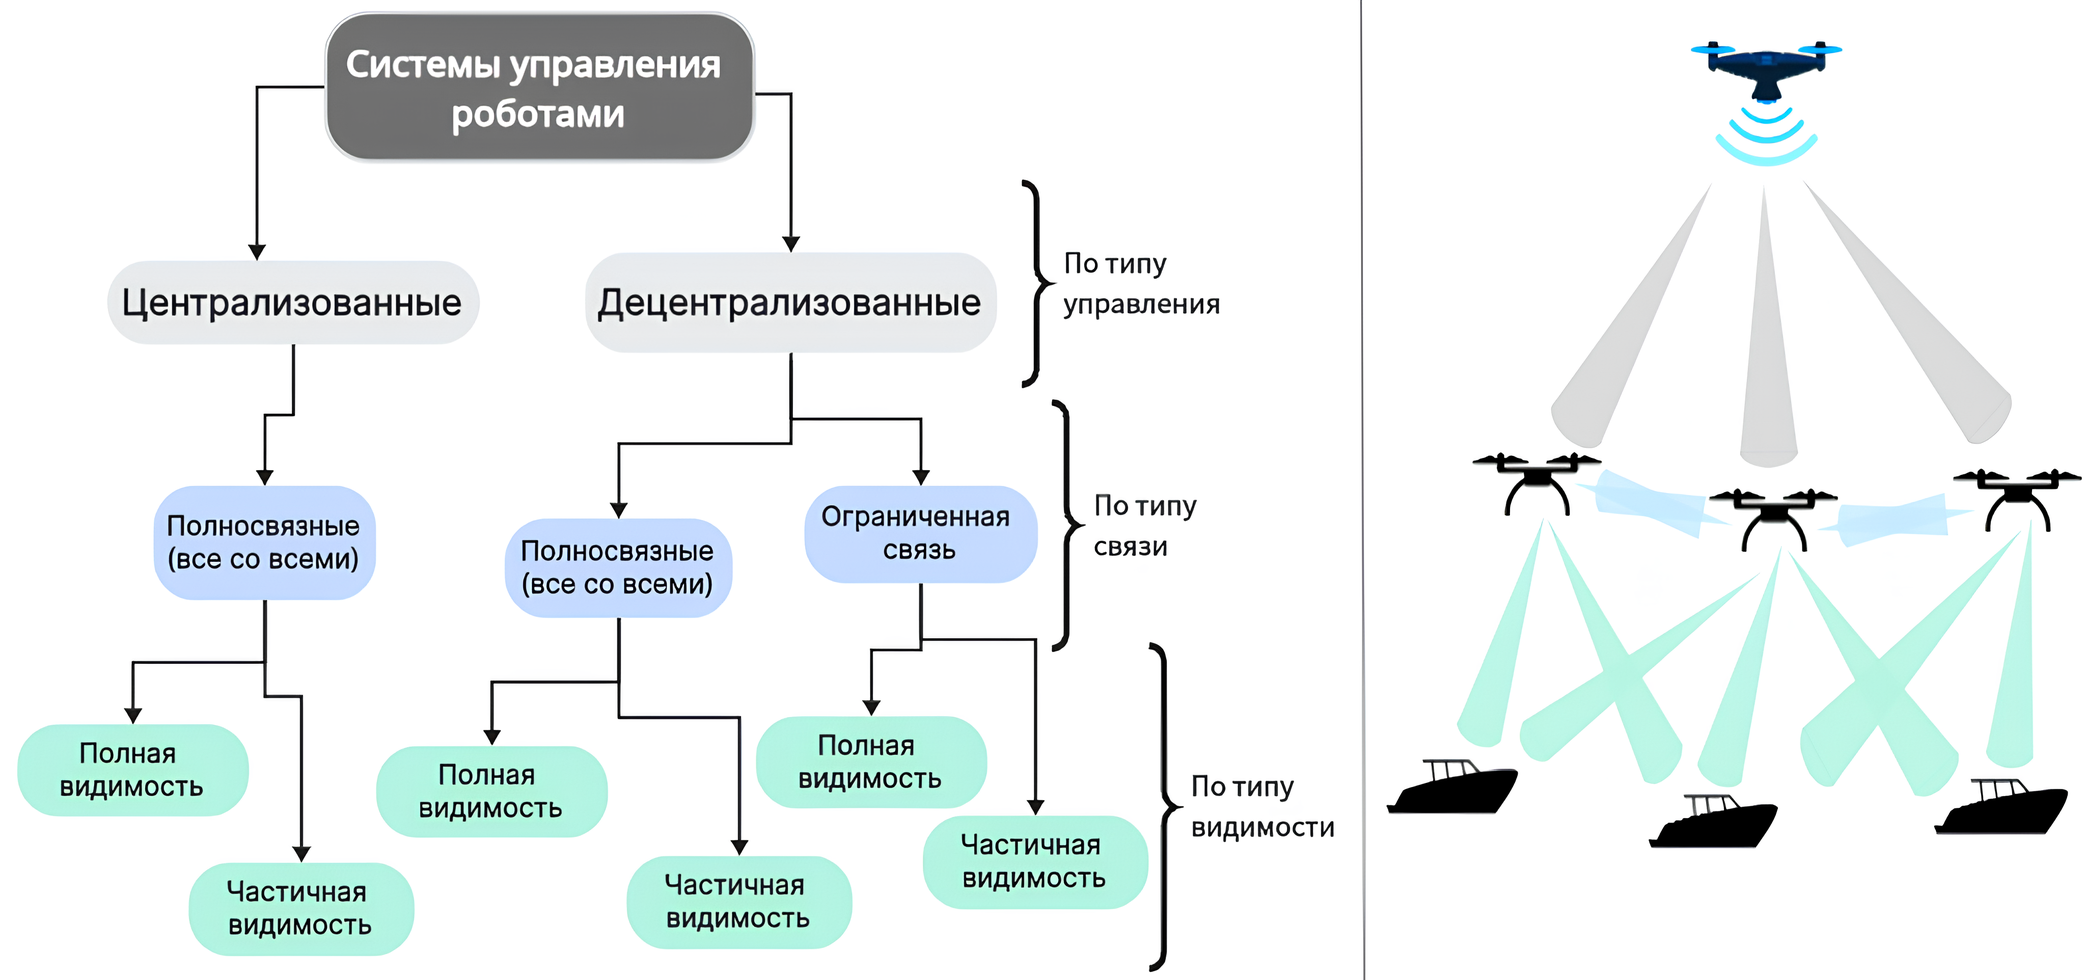
\includegraphics[width=\textwidth,height=0.95\textheight,keepaspectratio]{classification.png}
	\end{frame}


	\begin{frame}
		\frametitle{Положения, выносимые на защиту}
		\begin{itemize}
			\item Принятые допущения:
				\begin{itemize}
					\item Все роботы имеют одинаковый и неизменный радиус связи
					\item Все роботы обладают одинаковыми скоростями движения
					\item Каждый робот видит все цели
					\item Точность определения координат целей одинакова для всех роботов
					\item Не учитываются динамические системы роботов
				\end{itemize}
			\item Постановка задачи
			\item Итерационный децентрализованный алгоритм назначения целей роботам:
				\begin{itemize}
					\item Учет ограничений связи (R)
					\item Управление точностью решения через параметр (\(\varepsilon\))
				\end{itemize}
			\item Результаты исследований
			\item Выводы о применимости
		\end{itemize}
	\end{frame}

	\begin{frame}{Формальная постановка задачи}
		\vspace*{-0.2cm}
		\small
		\textbf{Дано:}
		\begin{itemize}
			\item Множество роботов $R = \{r_1, r_2, \ldots, r_n\}$.
			\item Множество целей $T = \{t_1, t_2, \ldots, t_m\}$.
			\item Матрица выгод $A = \{\alpha_{ij}\}$, где $\alpha_{ij}$ --- выгода от назначения робота $i$ цели $j$.
		\end{itemize}
		
		\textbf{Цель:} Максимизировать суммарную выгоду
		\[
		\sum_{i=1}^n \alpha_{i j_i} \rightarrow \max,
		\]
		где $j_i$ --- цель, назначенная роботу $r_i$.
		

		\vspace*{0.1cm}
		\textbf{Ограничения:}
		\begin{itemize}
			\item Каждый робот получает не более одной цели: $\sum_{j=1}^m x_{ij} \leq 1, \ \forall i = 1, \ldots, n$.
			\item Каждая цель назначается не более чем одному роботу: $\sum_{i=1}^n x_{ij} \leq 1, \ \forall j = 1, \ldots, m$.
			\item $x_{ij} \in \{0, 1\}$, где $x_{ij} = 1$, если робот $i$ назначен цели $j$, иначе $x_{ij} = 0$.
		\end{itemize}
	
	\end{frame}

	

	\begin{frame}
		\frametitle{Венгерский метод}
		\begin{columns}[T] % Параметр T выравнивает колонки по верху
			\begin{column}{0.5\textwidth} % Левая колонка (текст)
				\begin{itemize}
					\item Единый центр управления (централизованный подход)
                   				 \item Гарантирует точное оптимальное решение
                   				 \item Вычислительная сложность: $O(n^2 * m)$
				\end{itemize}
			\end{column}
			\begin{column}{0.5\textwidth} % Правая колонка (изображение)
				\centering
				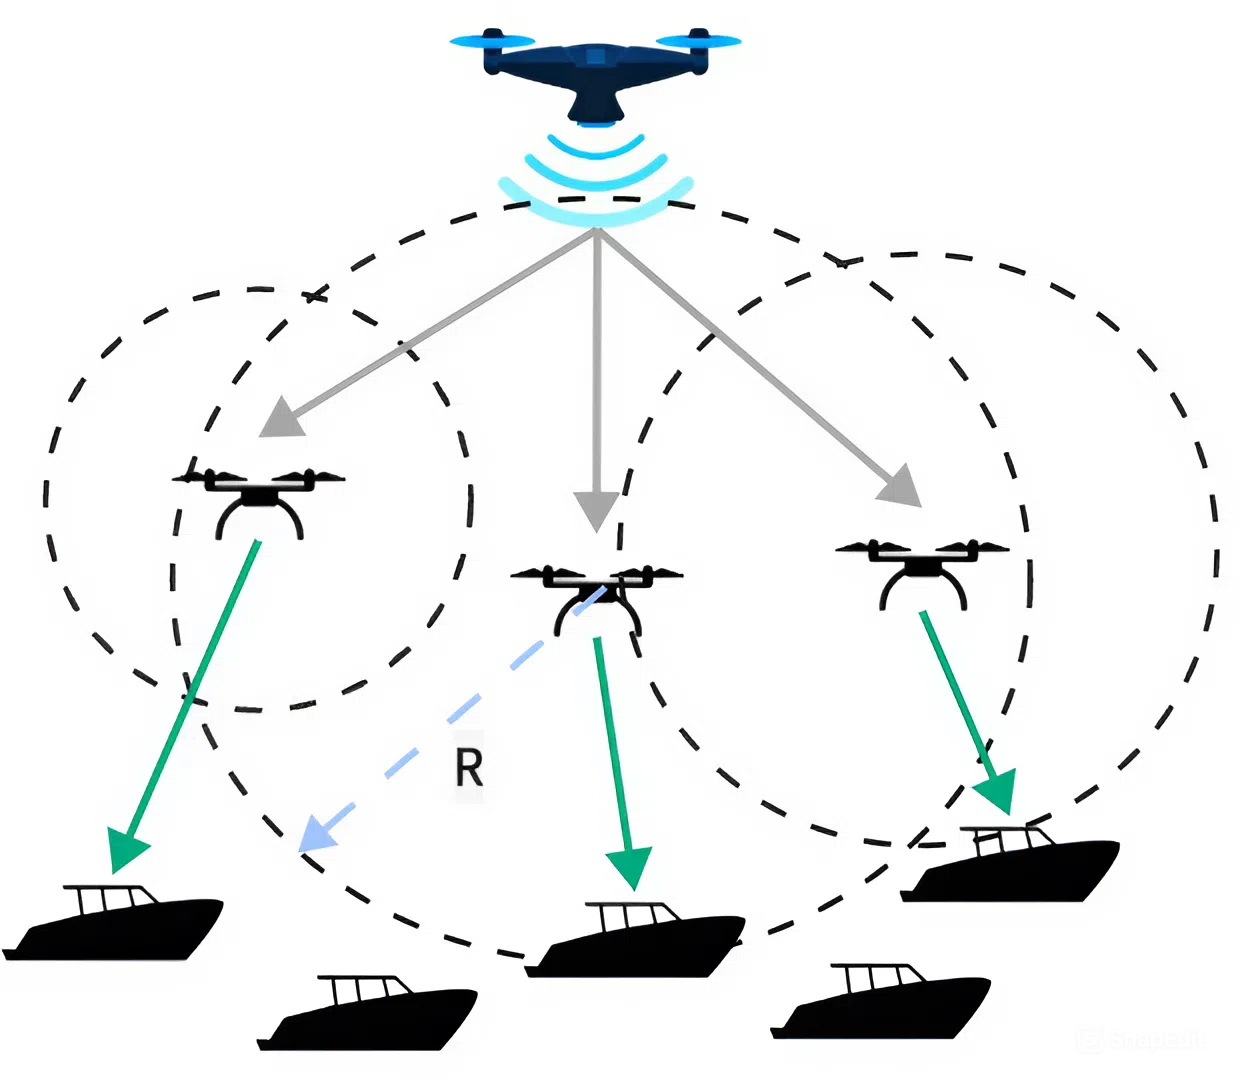
\includegraphics[width=\textwidth,height=0.85\textheight,keepaspectratio]{mrta2.jpeg}
			\end{column}
		\end{columns}
	\end{frame}
                

	\begin{frame}
	    \frametitle{Алгоритм аукциона}
	    \begin{columns}[T]
	        \begin{column}{0.6\textwidth}
	            \begin{itemize}
	                \item Нет единого центра управления
	                \item Имитирует процесс торгов
	                \item Параметр \(\varepsilon\) контролирует точность
	                \item Требует полной связи между роботами
	                \item Число итераций $\sim m\cdot C/$\(\varepsilon\)
	            \end{itemize}
	        \end{column}
	        \begin{column}{0.4\textwidth}
	            \hspace*{-1cm} % Отрицательный отступ для смещения влево
	            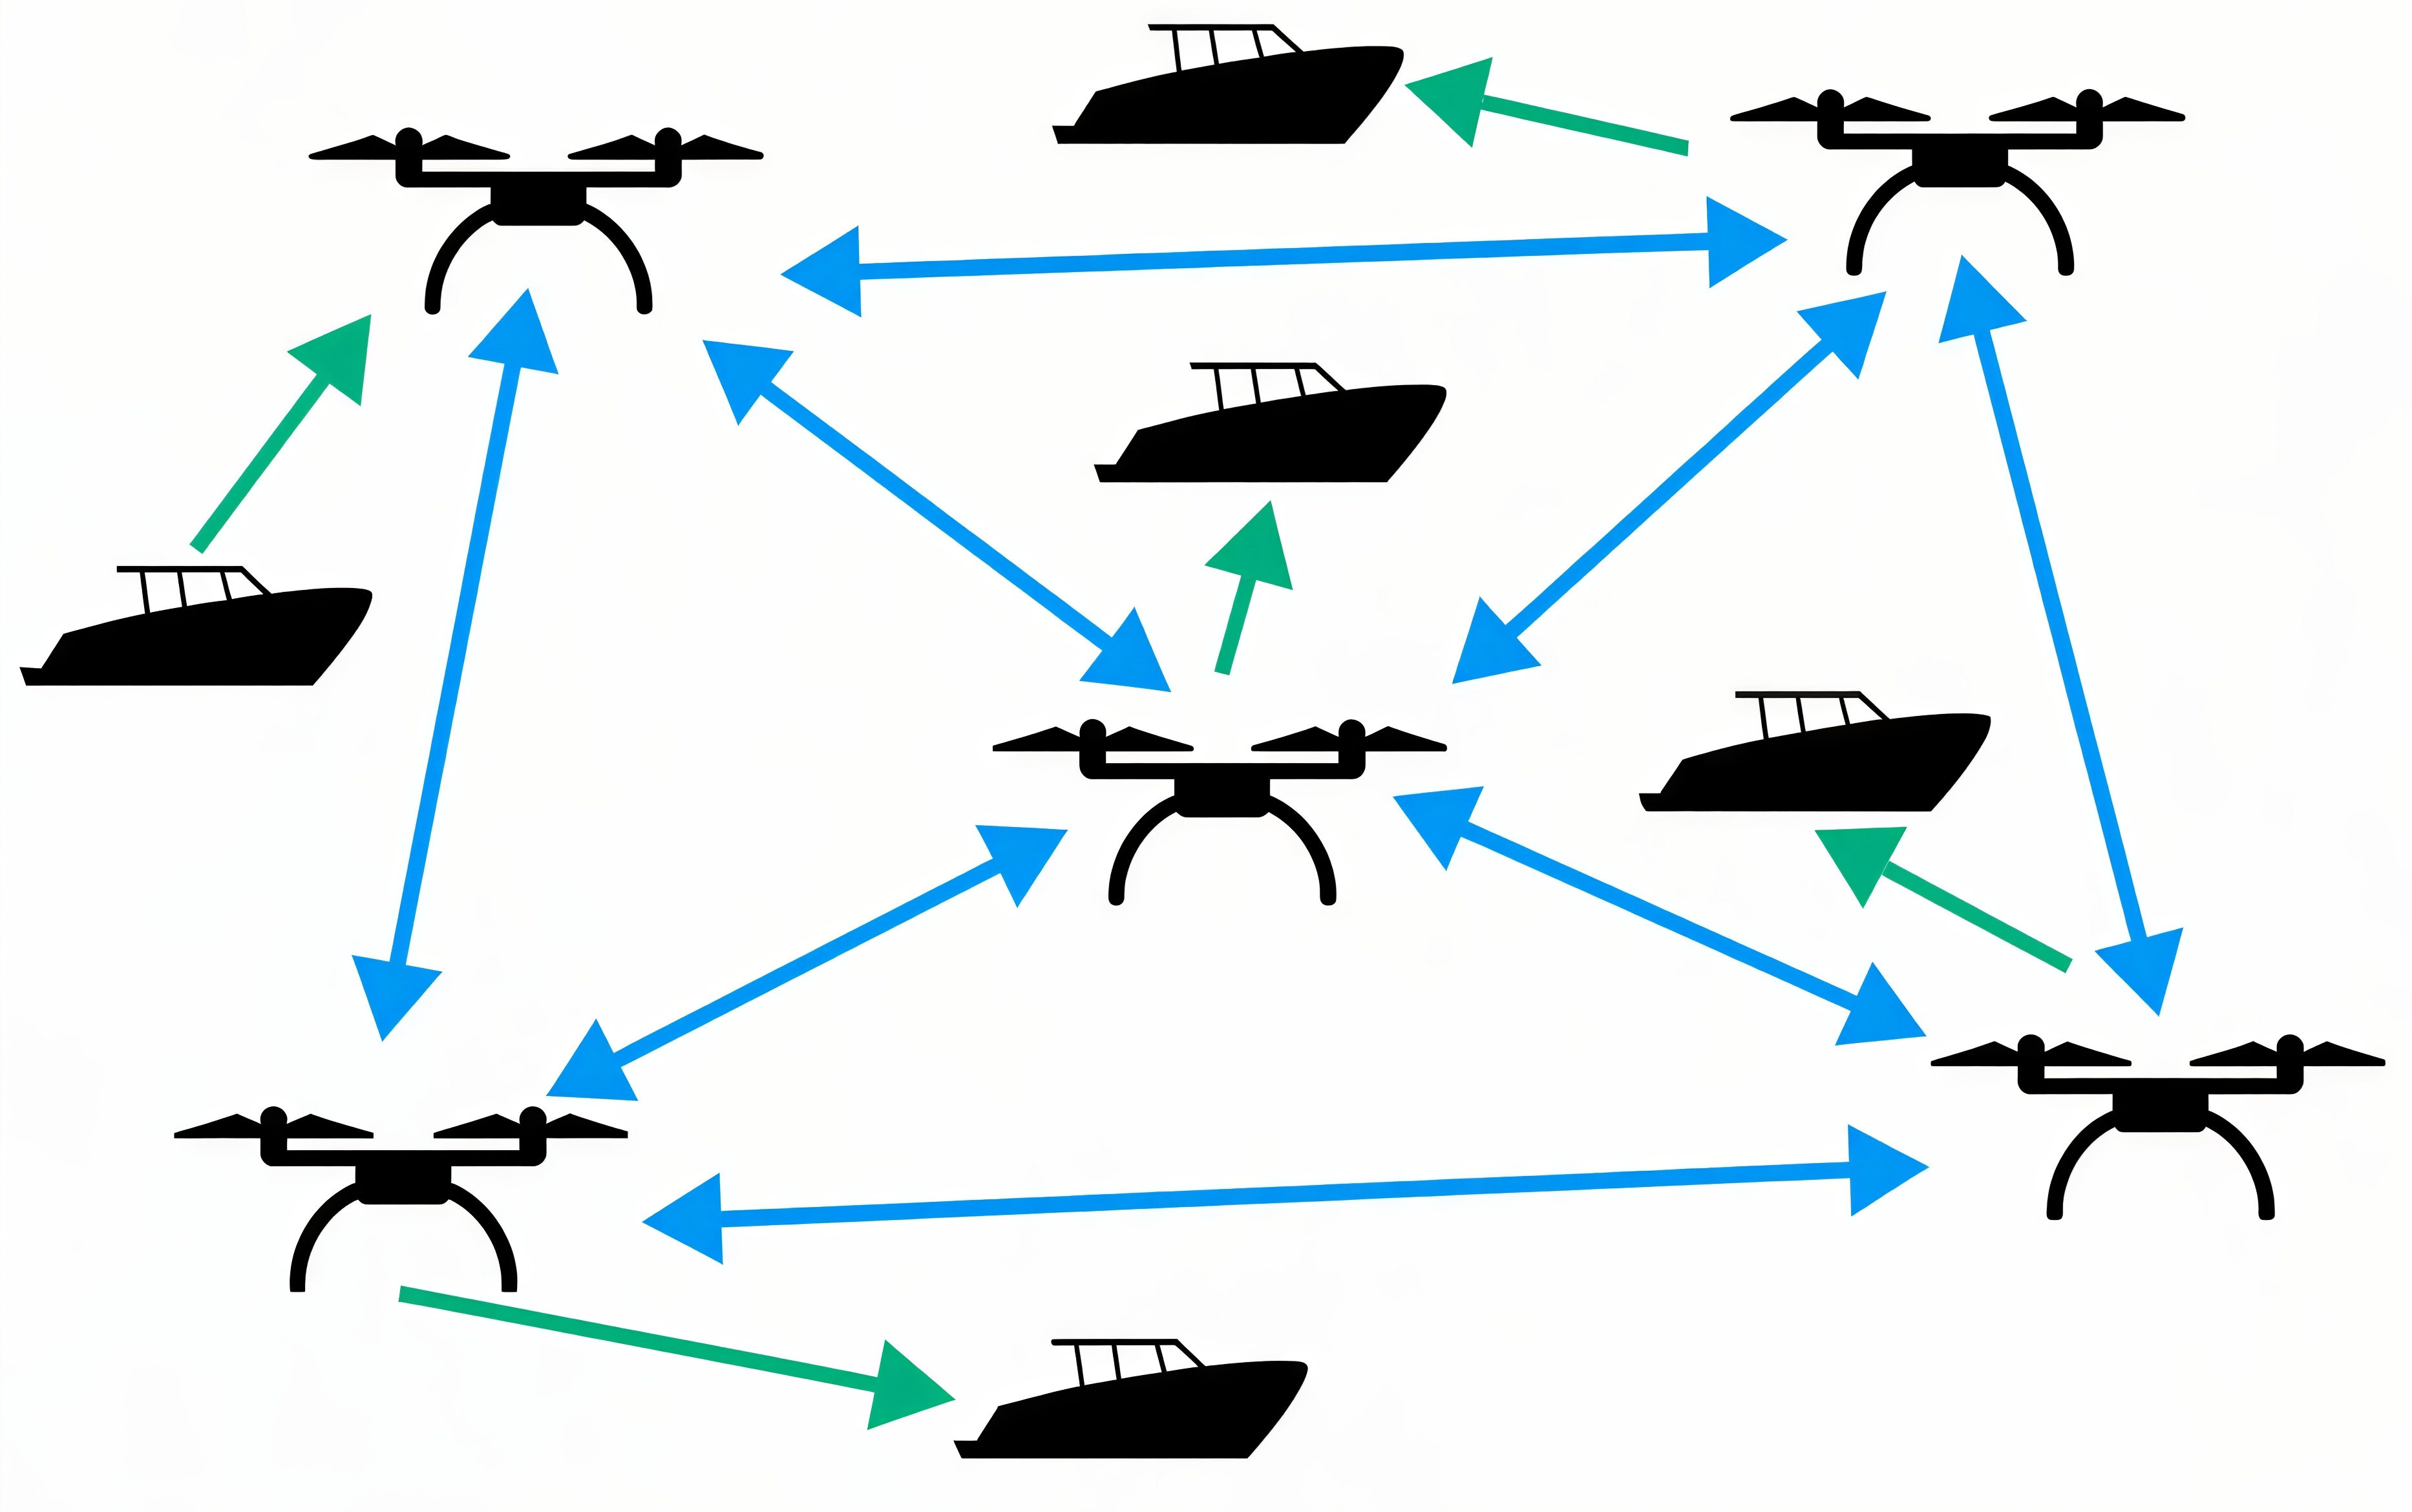
\includegraphics[width=1.2\textwidth,height=0.85\textheight,keepaspectratio]{mrta3.jpeg}
	        \end{column}
	    \end{columns}
	\end{frame}

	
	\begin{frame}
		\frametitle{Описание аукционного алгоритма}
			
			\begin{itemize}
				\item \textbf{Инициализация}: 
				\begin{itemize}
					\item Установить цены целей: \( p_j = 0, \ \forall j \).
					\item Назначения роботов пустые.
				\end{itemize}
				\item \textbf{Итерация для каждого робота} \( i \):
				\begin{itemize}
					\item Выбрать цель: \( j_i = \arg\max_j \{\alpha_{ij} - p_j\} \) (макс. выгода).
					\item Вычислить: 
					\begin{itemize}
						\item \( v_i = \max_j \{\alpha_{ij} - p_j\} \) (макс. выгода).
						\item \( w_i = \max_{j \neq j_i} \{\alpha_{ij} - p_j\} \) (вторая по величине выгода).
					\end{itemize}
					\item Переназначить робота \( i \) на цель \( j_i \).
					\item Обновить цену: \( p_{j_i} \gets p_{j_i} + (v_i - w_i + \varepsilon) \).
				\end{itemize}
				\item \textbf{Условие завершения}: Все роботы «почти счастливы».
				\item \textbf{«Почти счастье»}: 
				\[ \alpha_{i j_i} - p_{j_i} \geq \max_j \{\alpha_{ij} - p_j\} - \varepsilon.\]
			\end{itemize}
	\end{frame}


	\begin{frame}
		\frametitle{Модификация алгоритма аукциона}
		\begin{columns}[T] % Параметр T выравнивает колонки по верху
			\begin{column}{0.6\textwidth} % Левая колонка (текст)
				\begin{itemize}
					\item Нет единого центра управления
					\item Ограниченная связь между роботами (внутри связных компонент)
					\item Полная видимость целей для всех роботов
					\item Разделение роботов на связные компоненты по графу связи
					\item Независимый аукцион в каждой компоненте
				\end{itemize}
			\end{column}
			\begin{column}{0.4\textwidth} % Правая колонка (изображение)
				\centering
				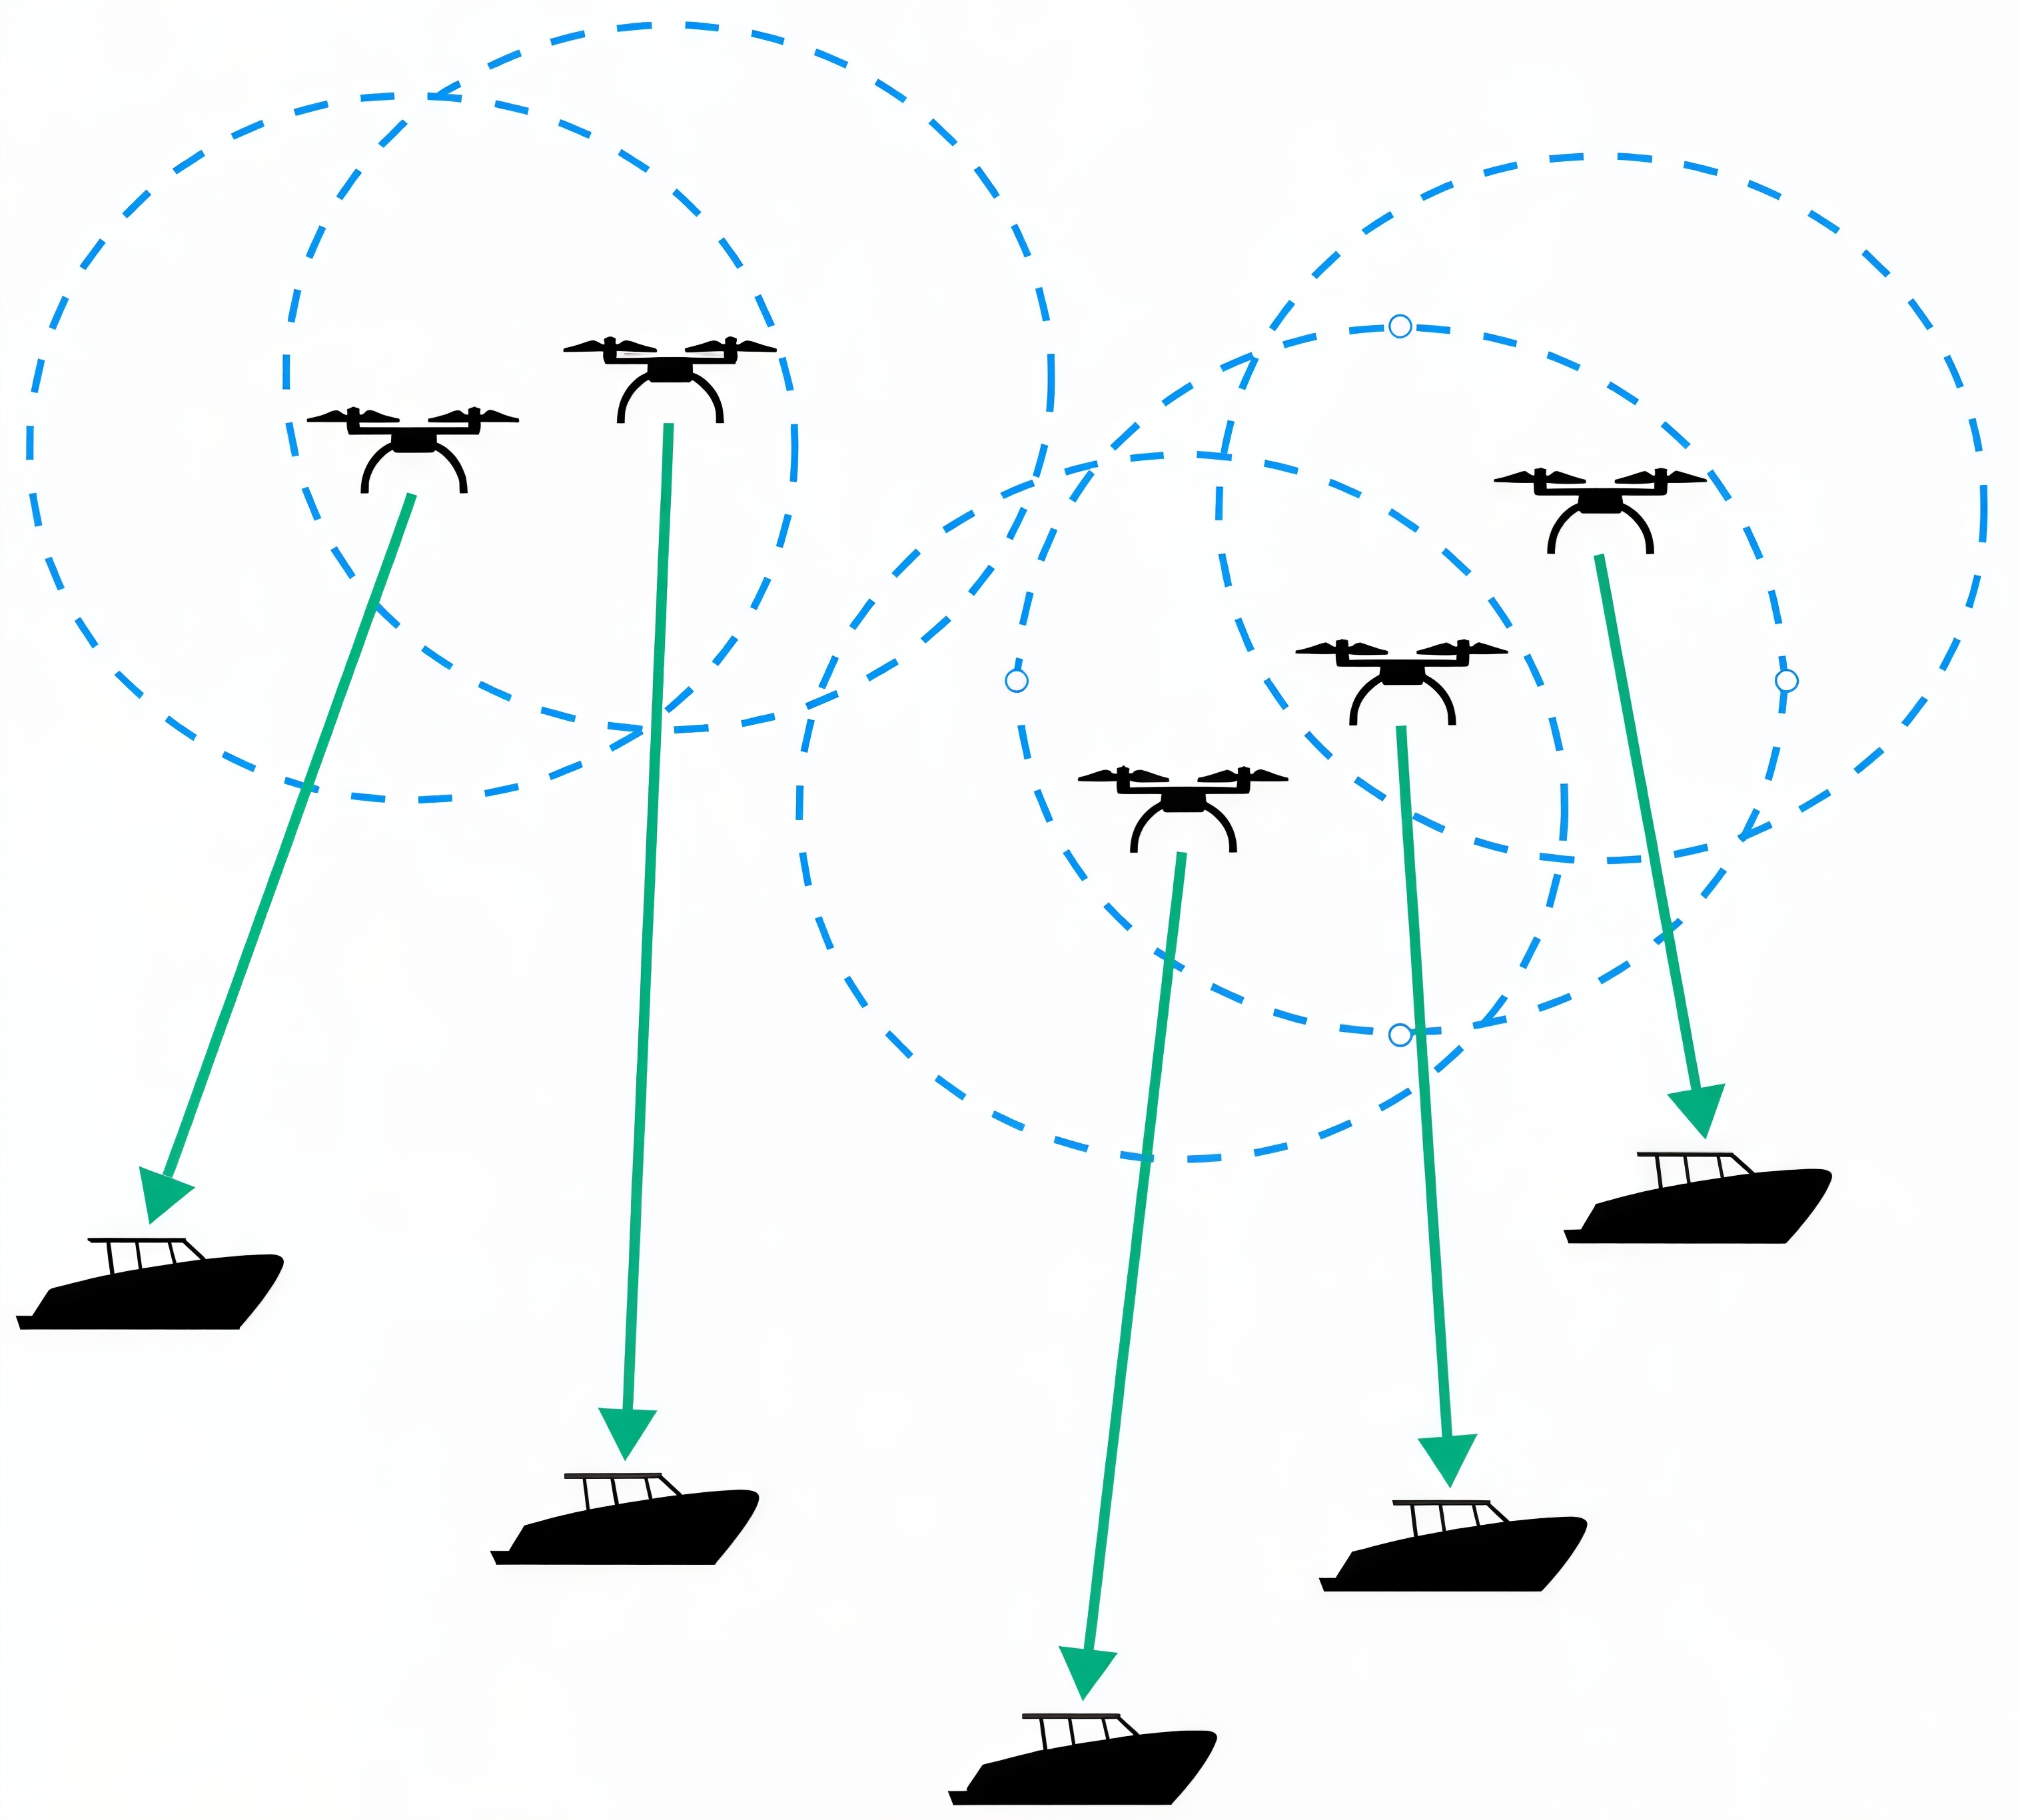
\includegraphics[width=\textwidth,height=0.85\textheight,keepaspectratio]{mrta4.jpeg}
			\end{column}
		\end{columns}
	\end{frame}
	
	\begin{frame}
		\frametitle{Результаты экспериментов}
	\end{frame}
	
	\begin{frame}
		\frametitle{Выводы и перспективы}
	\end{frame}
	
\end{document}